\section{Summary of Metrics}\label{analysis}

Some fundamental metrics are based simply on counting the number of interactions or the lines of code of a class as shown in Section \ref{related}. Next, we take a closer look at the most famous object-oriented metrics, the "CK-metrics". It is a set of metrics proposed by Chidamber and Kemerer in 1991 specifically for object-oriented software \cite{b15chidamber1991towards}. Build on the basic metrics table of the Chapter \ref{related}, divided in class metrics, method metrics and attribute metrics, more detailed aspects are now examined. 

Many metrics are based on comparable ideas and provide redundant information. By using a subset of metrics, prediction models can be built to identify the classes that are in fault. In the table \ref{tab:metrics}, on can see the CK-metrics summarized, which are named in many other papers too.

\begin{table}
	\caption{The CK Metrics.}~\label{tab:metrics}
	
	\setlength\tabcolsep{3pt}
	\renewcommand{\arraystretch}{1.4}% for the vertical padding
	\begin{tabularx}{\columnwidth}{ | c | p{5.6cm} || c | }
		\hline
		Abbrevation & Definition & Sources \\ \hline\hline
		\textbf{CBO} & Coupling between objects for a class is a count of the number of non-inheritance related couples with other classes & \cite{b15chidamber1991towards, b1aggarwal2007investigating, b3al2012fault} \\ \hline
		\textbf{LCOM} & Lack of Cohesion in Methods counts number of null pairs of methods that do not have common attributes & \cite{b15chidamber1991towards, b1aggarwal2007investigating} \\ \hline
		\textbf{NOC} & The number of children is the number of subclasses of a child class in a hierarchy & \cite{b15chidamber1991towards, b1aggarwal2007investigating} \\ \hline
		\textbf{DOI} & The depth of a class within the inheritance hierarchy is the maximum number of steps from the class node to the root of the tree and is measured by the number of ancestor classes & \cite{b15chidamber1991towards, b1aggarwal2007investigating} \\ \hline
		\textbf{WMC} & The weighted methods per class is a count of sum of complexities of all methods in a class & \cite{b15chidamber1991towards, b1aggarwal2007investigating} \\ \hline
		\textbf{RFC} & The response set of a class is defined as set of methods that can be potentially executed in response to a message received by an object of that class & \cite{b15chidamber1991towards, b1aggarwal2007investigating} \\ \hline
	\end{tabularx}
\end{table}

Next, some of the CK metrics will be presented in more detail and with some examples.

\subsubsection{\textbf{CBO}}: The coupling between objects for a class is a count of the number of non-inheritance related couples with other classes. Two things are coupled if and only at least one of them atcs upon the other. Any evidence of a method of one object using methods or instance variables of another object constitutes coupling. Given is an example for CBO: 

\begin{small}
\begin{verbatim}
import java.util.Calendar;
	
public class AdultIssuePolicy implements
	                              IssuePolicy {
   public Calendar compute(BiblioType type, 
   								Calendar from) {
      Calendar res = (Calendar)from.clone();
        res.add(Calendar.DATE, 14);
        return res;
   }
}
\end{verbatim}
\end{small}

Note, that coupling is not associative, i.e., if $A$ is coupled to $B$ and $B$ is coupled to $C$, this does not imply that $C$ is coupled to $A$.

\subsubsection{\textbf{LCOM}}: The Lack of Cohesion in Methods counts number of null pairs of methods that do not have common attributes. Consider a Class $A$ with methods $m_1$, $m_2$,...$m_n$. Let $\{I_i\} =$ set of instance variables used by the method $m_i$. There are $n$ such sets $I_1$,...,$I_n$. The LCOM is therefore the number of disjoint sets formed by the intersections of the $n$ sets. Formally let´s say a Class $C$ with 
\begin{itemize}
	\item $k$ fields $f_1,f_2,...,f_k$ and
	\item $n$ public methods $m_1,m_2,m_3,...,m_n$.
\end{itemize} 
So $I_i= \{f_l:f_l$ is used by $m_i\}$ and $N=\frac{n(n-1)}{2}$ is the number of different possible pairs of methods. It follows that

\begin{displaymath}
	P=|\{(m_i,m_j):i<j \ and \ I_i \cap I_j = \emptyset\}
\end{displaymath}  
\begin{displaymath}
	Q=|\{(m_i,m_j):i<j\ and \ I_i \cap I_j \neq \emptyset\}
\end{displaymath} 

and $N=P+Q$. The LCOM is $P$. Given is an example for LCOM:

\begin{small}
\begin{verbatim}
public class A {
  private int f1;
  private int f2;
  private int f3;
  private int f4;
  public void method1() { I1 = { f1, f2 }
     // uses f1
     // uses f2
  }
  public void method2() { I2 = { f2, f3 }
     // uses f2
     // uses f3
  }
  public void method3() { I3 = { f3, f4 }
     // uses f3
     // uses f4
  }
}
\end{verbatim}
\end{small}

When looking at the $(m_i,m_j)$ pairs, the $I_i \cap I_j$ of $(method1,method2)$ is $_f2$, $(method1,method3)$ is $\emptyset$ and $(method2,method3)$ is $_f3$. Therefore LCOM is $1$.

\subsubsection{\textbf{NOC}} The number of immediate subclasses subordinated to a class in the class hierarchy, which is pretty much self explanatory.

\subsubsection{\textbf{DOI}} The Depth of inheritance of the class is the depth of inheritance tree metric for the class, it is the length of the longest path to the root. The deeper a class is in the hierarchy, the greater the number of methods it is likely to inherit, making it more
complex, but it is useful to have a measure of how deep a particular class is in hierarchy so that the class can be designed with reuse of inherited methods.

\subsubsection{\textbf{WMC}} The Weighted Methods Per Class is a count of sum of complexities of all methods in a class. Consider a Class $C$ with methods $m_1,m_2,...,m_n$. Let $c_1,..,c_n$ be the static complexity if the methods. Then 
\begin{displaymath}
	WMC = \sum_{i=1}^{n} c_1.
\end{displaymath}

\subsubsection{\textbf{RFC}} the Response For a Class is defined as set of methods that can be potentially executed in response to a message received by an object of that class. The RFC $=|RS|$ where $RS$ is the response set for the class. The response set if an object $\equiv \{$set of all methods that can be invoked in response to a message to the object$\}$. Given is an example for RFC:

\begin{small}
\begin{verbatim}
public class A {
   private B aB;
   public void methA1() {
      return aB.methB1();
   }
   public void methA2(C aC) {
      return aC.methC1();
   }
}
\end{verbatim}
\end{small}

It follows $RS = { methA1, methA2, methB1, methC1}$.

These metrics are the fundamental rules, that developers follow. People who investigate new studies on metrics in objectorineted systems usually have these rules as a cornerstone.
Some issues that comes with this metrics, are what happen with classes with no fields, static member or self calls. Not all questions, provide the metrics answer, they just provide a framework.

Next step, is the look at a study that deals with class cohesion metrics. After that, a bayesian network is explained, which is a bit more difficult.


\subsection{Method-Method Interaction-Based Cohesion Metrics for Object-Oriented Classes}\label{mmi}

Basic units of design in object-oriented programs are classes. Class cohesion refers to the relatedness of class members, i.e., their attributes and methods. Multiple metrics for class cohesion have been proposed in the literature. These object-oriented metrics are based on information available during the high-level or low-level design phases.
A formula that accurately measures the degree of interaction between each pair of methods is proposed and used as the basis for introducing a low-level design class cohesion (LSCC) metric \cite{b8al2012precise}. Low-level design (LLD) cohesion metrics use more finely resolved information than that used by High-level design (HLD) cohesion metrics. HLD cohesion metrics identify potential cohesion issues early in the HLD phase. 
In figure \ref{fig1}, rectangles represent methods, circles indicate attributes, and links illustrate the use of attributes by methods of a class. Metrics based on counting the number of links, i.e., the use of attributes by a method, can indicate whether a class is strongly or weakly cohesive. This finely granulated information is important to help software developers refactoring their code and detecting which methods to possibly remove, i.e., the methods that exhibit even no links with other methods. When a method-method interaction (MMI) metric is applied to measure the cohesion for the class shown in figure \ref{fig1}, the connectivity between each pair of methods is calculated, and it is clearly seen that method $m_3$ is weakly interconnected to other methods in this class.

\begin{figure}[htbp]
	\centerline{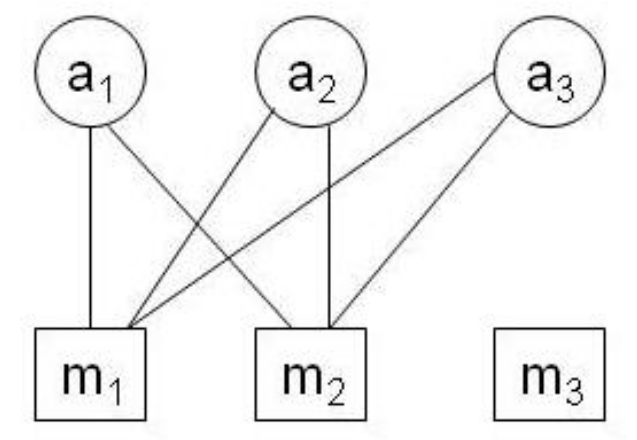
\includegraphics[width=0.2\textwidth]{pictures/am.png}}
	\caption{Sample representative graph for a hypothetical class \cite{b3al2012fault}.}
	\label{fig1}
\end{figure}

As shown in figure \ref{fig2}, there are four other classes with a different method-method interconnection. The class cohesion (CC) of Bonja and Kidanmariam is the ratio of the summation of the similarities between all pairs of methods to the total number of pairs of methods \cite{bonja2006metrics}. The similarity between methods $i$ and $j$ is defined as
\begin{displaymath}
	sim(i,j)=\frac{|I_i \cap I_j|}{|I_i \cup I_j|} ,  
\end{displaymath}
where $I_i$ and $I_j$ are the sets of attributes linked by methods $i$ and $j$, respectivly \cite{b3al2012fault}. In contrast with the class cohesion metric of Pena (SCOM), the calculation is defined as follows
\begin{displaymath}
	sim(i,j)=\frac{|I_i \cap I_j|}{min(|I_i|, |I_j|)} \cdot \frac{|I_i \cup I_j|}{n},  
\end{displaymath}
where $n$ is the number of attributes \cite{fernandez2006sensitive}.
Both CC and SCOM neither consider transitive MMI nor account for inheritance or different method types, and they have not been empirically validated against external quality attributes such as fault occurrences. Of course, there are many other metrics of this kind but the results for the metrics that consider the degree of interaction between each pair of methods are very close to each other \cite{b8al2012precise}.

\begin{figure}[htbp]
	\centerline{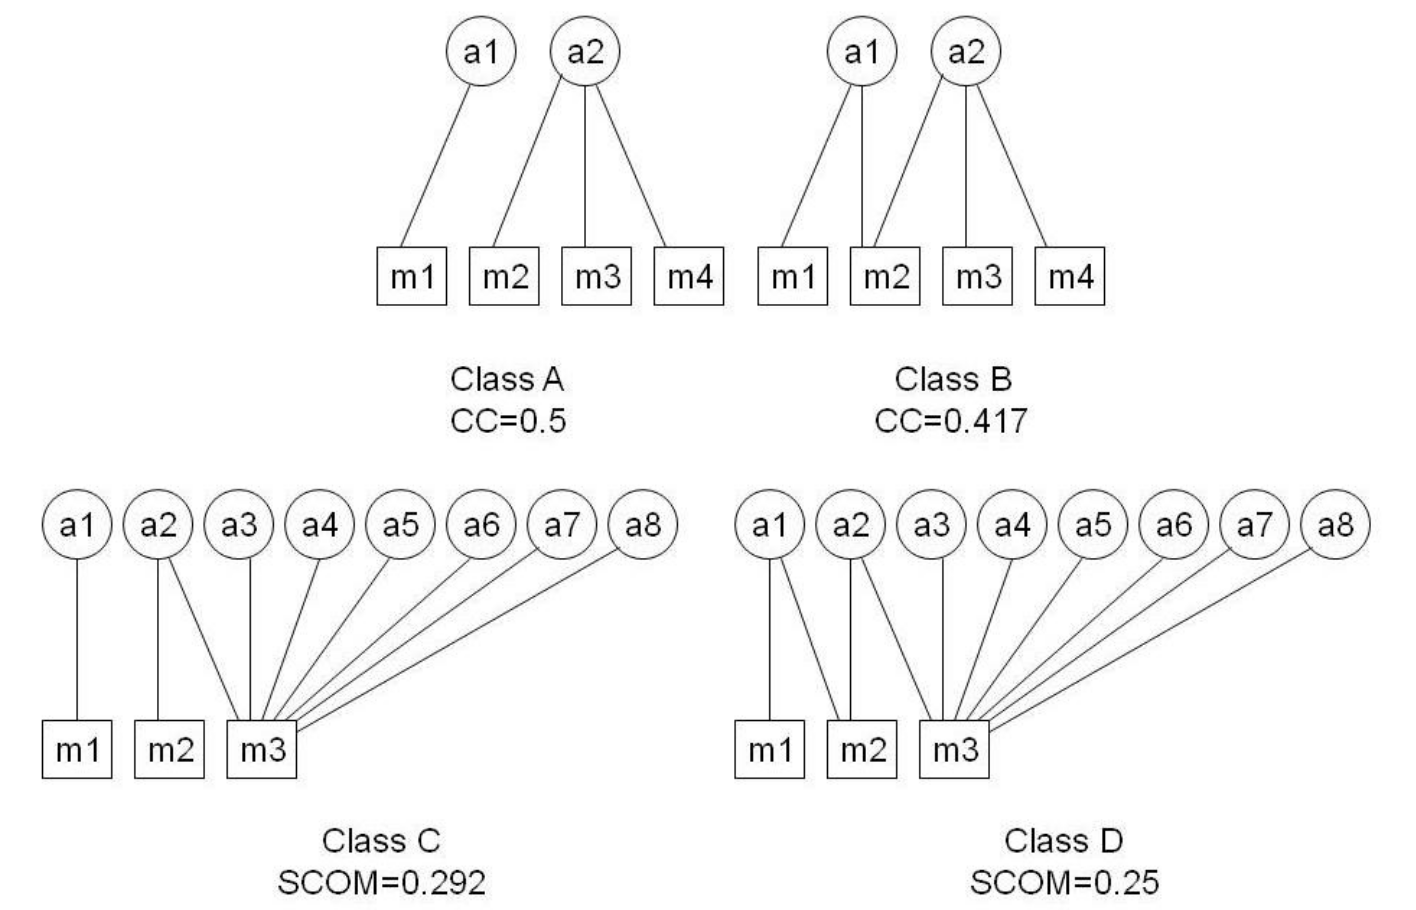
\includegraphics[width=0.4\textwidth]{pictures/am2.png}}
	\caption{Classes with different method-method connectivity patterns \cite{b3al2012fault}.}
	\label{fig2}
\end{figure}

The results suggest that class quality, as measured in terms of fault occurrences, can be more accurately explained by cohesion metrics that account for the degree of interaction between each pair of methods. The fault prediction of interconnection-based object-oriented class cohesion metrics should help the developer to support refactoring during the LLD phase, therefore in an early state of development \cite{b8al2012precise}.


\subsection{A Bayesian Network}

Some metrics are based on the concept of the possibility that the methods and attributes of a class of the code can be presented as a graph. Here the interaction can be graphically represented by an undirected edge that links a circular node (attribute) to a rectangular node (method).

The next method to take a closer look at the fault-proneness is a concise representation of a joint probability distribution on a set of statistical variables. Bayesian methods can be used for assessing software fault content and fault proneness. A bayesian network (BN) is encoded as an acyclic graph of nodes and directed edges \cite{b9pai2007empirical}. Assuming that the relationship can be modeled with a general linear model, the structural and numerical specification for the BN is derived. The model can be thought of as a generalization of existing techniques for assessing software quality. The model consists roughly of two parts, first the method produces a probability distribution of the estimated fault content per class in the system and second the conditional probability that a class contains a fault. 
The structure of the model is a BN model whose underlying representation is the generalized linear model. The definition probabilistic network (acyclic graph $G=(V,E)$; A set $S$, of (prior) conditional probability distributions).
Consider a finite set of random variables $X=\{X_1,X_2,....,X_n\}$. It can be defined that a probabilistic network $N=(G,X) over X$ consists of
 \begin{enumerate}
 	\item[-] a directed acyclic graph $G=(V,E)$, $V$ is the set of nodes in the graph and there is a one-one correspondence between $V$ and $X$. $E \subseteq V \times V$ the set of directed edges, representing conditional independence assumptions, i.e., for each $X_i \in X$, $i(X_i,N D_{x_i}| Pa_{x_i})$ and $N D_{x_i} = X \backslash ({X_i} \cup Des_{x_i})$ 
 	\item[-] a set of (prior) conditional probability distributions, that specifies $p(X_i)| p(Pa_{x_i})$ for each $X_i \in X$, where $Pa_{x_i}$ represents the set of immediate parents of $X$.
 \end{enumerate} 

Once a network is specified over a set of random variables, their marginal and joint probabilities can be computed.
Given a BN structure, the joint probability distribution over $X$ is encoded as

\begin{displaymath}
	p(X)= \prod_{i=1}^{n}p(X_i|P_{ax_i})
\end{displaymath}

And given this joint probability, the marginal probability of a random variable $X_i$ is computed as 

\begin{displaymath}
	p(X_i)= \sum_{X_i,j\neq i}^{n}p(X)
\end{displaymath}

The CK metrics mentioned in the previous section can be found here, too. The model parameters that are used are listed in the following \cite{b9pai2007empirical}: 

\begin{itemize}
	\item[1.] Weighted methods per class (WMC)
	\item[2.] Depth of inheritance tree (DOI)
	\item[3.] Response for class (RFC)
	\item[4.] Number of children (NOC)
	\item[5.] Coupling between object classes (CBO)
	\item[6.] Lack of cohesion in methods (LCOM)
	\item[7.] Source lines of code (SLOC): This is measured as the total lines of source code in the class and serves as a measure of class size.
\end{itemize}

As can be seen the parameters 1.-6. are the CK metrics \ref{tab:metrics}. The 7. point is already presented in table \ref{tab:classmetrics}, too.
The dependent variables, which serve as surrogate metrics of software quality here, are
\begin{itemize}
	\item Fault Content (\textbf{FC}): We define fault content as the number of faults per class. The estimation of our model is a (marginal) conditional probability of observing a certain number of faults per class, given the metrics for that class.
	\item Fault proneness (\textbf{FP}): The conditional probability that a class contains a fault, given the metrics for that class.
\end{itemize}

In this approach, it is assumed that a general linear model (GLM) relates the dependent and independent random variables and construct a BN structure that represents the GLM. This assumption is motivated by several factors: The GLM is versatile enough to represent existing linear relationships or, through transformations, a variety of nonlinear relationships. Linear models also provide a relatively simple and parameterized way to capture the dependencies between domain variables. 
 
Consider that a responsive variable $Y$ varies as some function of a set $X=\{X_1,X_",...,X_k\}$ of independent predictor variables. In the GLM, it follows 
\begin{displaymath}
 	E(X)= \mu = g^{-1}(X\beta),
\end{displaymath}
where $Y$ is the set of observations with expected value $E(X)= \mu$. The linear predictor with coefficients $\beta$ is $X\beta$ and $g$ is the link function determined by the distribution of $Y$ as graphically shown in figure \ref{fig1bn}. 

\begin{figure}[htbp]
	\centerline{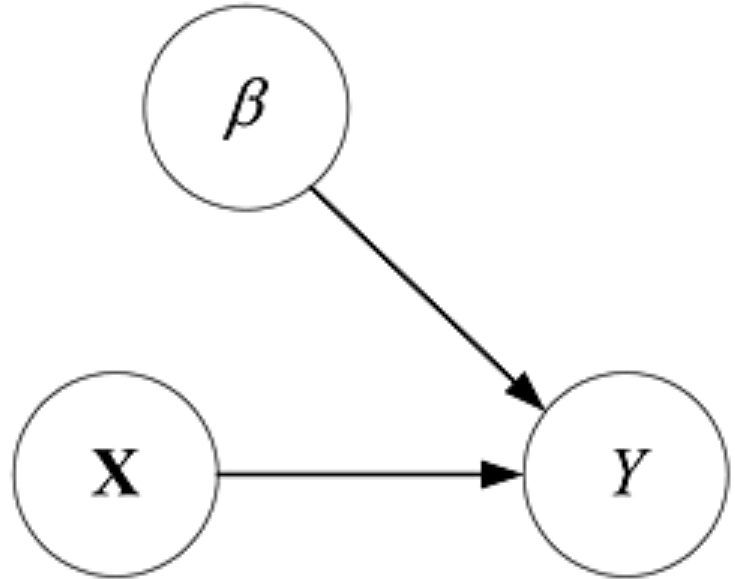
\includegraphics[width=0.2\textwidth]{pictures/bn1.png}}
	\caption{BN representation of a general linear model.}
	\label{fig1bn}
\end{figure}

Figure \ref{fig2bn} shows how the individual components of the model parameters influence the FC and FP. Here the connection between $X$ and $Y$ can be clearly seen.

\begin{figure}[htbp]
	\centerline{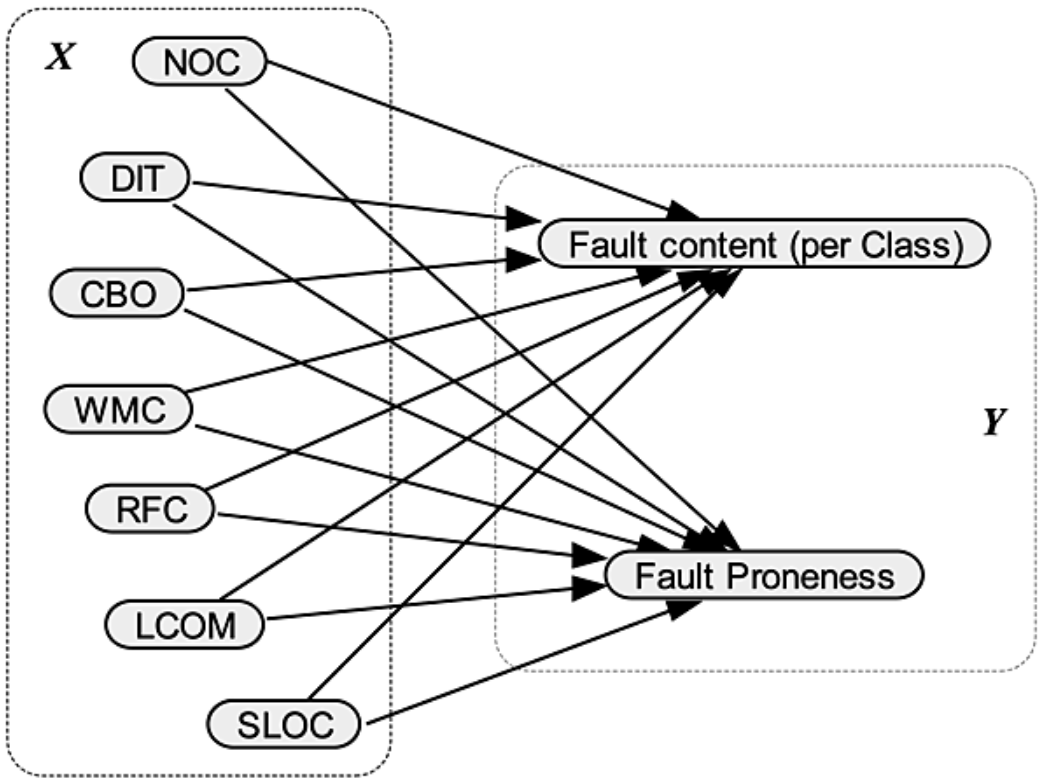
\includegraphics[width=0.4\textwidth]{pictures/bn2.png}}
	\caption{BN model for fault content and fault-proneness analysis.}
	\label{fig2bn}
\end{figure}

In table \ref{fig3bn}, the used data is given. After the set up model has gone through the data, one can see, that the SLOC is about $43K$ and the faulty percentage is nearly $40\%$, which is enormous. 
The results also show that this model produces these estimations at a statistically significant level. The results of performing multiple regression, the metrics WMC, CBO, RFC, and SLOC are very significant for assessing both fault content and fault proneness. In general this specific set of predictors is very significant for assessing FC and FP in large software systems.

\begin{figure}[htbp]
	\centerline{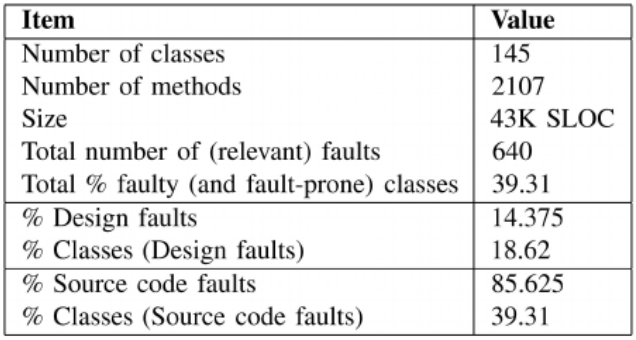
\includegraphics[width=0.45\textwidth]{pictures/tableBN.png}}
	\caption{Data Description.}
	\label{fig3bn}
\end{figure}